\appendix

\section{Appendix: Configuration and Reproducibility Notes}

\subsection{Project Status Summary}

Table~\ref{tab:status-appendix} summarizes the state of the components
referenced in the main text. The classifier and detector evidence are
sufficient to support the results in \S\ref{sec:results}; the
language-stage components remain in transition.

\begin{table}[H]
\centering
\caption{Status summary for the components referenced in this
manuscript.}
\label{tab:status-appendix}
\begin{tabularx}{\linewidth}{>{\raggedright\arraybackslash}p{0.33\linewidth} >{\raggedright\arraybackslash}p{0.13\linewidth} X}
\toprule
Component & Status & Notes \\
\midrule
Balanced holdout rebuild with provenance & Done & The active holdout now contains 20 images for each of the seven classes \\
Augmented class-floor balancing & Done & Underrepresented classes in the active augmented split were raised to a minimum of 300 images \\
ResNet v3 retrain on the balanced split & Done & The current classifier checkpoint is evaluated on the balanced 140-image holdout \\
Runtime promotion with rollback path & Done & The runtime app defaults to the current v3 checkpoint and keeps an explicit override path \\
p1/p2 runtime logging & Done & JSONL logging added for downstream calibration analysis \\
Tight dual-report generation pilot & Done & Focused 20-image pilot completed with 36 generated reports \\
Full stage-2 regeneration under tight policy & Pending & The current stage-2 JSON remains stale relative to the augmented training root \\
MiniGPT retrain on regenerated stage-2 & Pending & Current checkpoint predates the holdout carve and dual-report policy \\
Clean holdout explanation evaluation & Pending & No post-regeneration holdout explanation metric exists yet \\
RF-DETR on/off ablation on clean holdout & Pending & Planned but not executed \\
\bottomrule
\end{tabularx}

\end{table}

\subsection{Classifier Training and Calibration Details}

The deployed ResNet-50 checkpoint is trained on the rebuilt
\texttt{train\_aug} root described in \S\ref{sec:data} with standard
ImageNet normalization, moderate train-time augmentation, and a
256-pixel evaluation crop. The post-hoc temperature parameter
$T = 0.7513$ in Eq.~\ref{eq:tta-calibration} is fit by minimizing
negative log-likelihood on the internal validation
split~\citep{guo2017calibration}. Reliability bins are constructed on a
ten-bin equal-width partition of $[0,1]$, following the protocol used
in the calibration literature~\citep{naeini2015ece}.

\subsection{Grounding-Detector Training Configuration}

The RF-DETR Small grounding detector is fine-tuned from a publicly
released checkpoint with the following configuration:

\begin{itemize}[leftmargin=1.3em]
\item six-class plant-part vocabulary ($\mathrm{flower}, \mathrm{fruit},
\mathrm{leaf}, \mathrm{root}, \mathrm{soil}, \mathrm{stem}$);
\item COCO-format dataset with 753 train images / 19{,}487 train
annotations and 322 validation images / 8{,}582 validation annotations;
\item 100 training epochs at resolution 560;
\item batch size 8 with gradient accumulation factor 2 (effective
batch 16);
\item encoder learning rate $1.5\times 10^{-4}$, decoder learning rate
$1\times 10^{-4}$, weight decay $1\times 10^{-4}$;
\item cosine learning-rate schedule with five warmup epochs and minimum
learning-rate factor $0.01$;
\item drop-path $0.1$;
\item exponential moving average enabled;
\item seed 42;
\item per-class runtime thresholds $\theta_p$ tuned per part as listed
in \S\ref{sec:system}.
\end{itemize}

\subsection{Report-Writer Training Configuration}

The active MiniGPT-v2 training configuration is summarized below. These
values are repository-current settings; we reiterate that the deployed
checkpoint predates the constrained stage-2 redesign and the holdout
carve, and that retraining on the regenerated targets is identified as
pending in Table~\ref{tab:status-appendix}.

\begin{itemize}[leftmargin=1.3em]
\item image size 448 for both train and evaluation processors;
\item maximum text length of 500 tokens;
\item LoRA rank $r=64$, $\alpha=128$, dropout $0.05$;
\item initial learning rate $1\times 10^{-5}$, minimum
$5\times 10^{-6}$, warmup $1\times 10^{-6}$;
\item 20 epochs with linear warmup and cosine decay;
\item per-GPU batch size 2 with 8 gradient-accumulation steps;
\item 10\% auto-validation split;
\item seed 42.
\end{itemize}

\subsection{Runtime Decision Rule}

The deployed runtime applies threshold-only acceptance under
Eq.~\ref{eq:threshold-gate} with the per-class thresholds listed in
Eq.~\ref{eq:class-thresholds}, the default threshold of $0.55$ for any
unmapped class, and a post-prompt-assembly low-confidence guard that
demotes accepted predictions whose top-1 probability falls below
$0.50$. The margin threshold of $0.08$ is recorded to the structured
decision log but is not currently activated as a runtime demotion rule;
its operating point will be calibrated from production decision logs.

\subsection{Scope of the Ambiguity Policy}

The constrained dual-report policy of \S\ref{sec:dualpolicy} is a
dataset-construction policy. It does not at present imply a user-facing
behavior in which the deployed report writer presents alternatives to
end users. A user-facing alternative-presentation feature would require
both a retrained MiniGPT-v2 checkpoint on regenerated targets and a
clean holdout explanation evaluation, both of which are listed as
pending in Table~\ref{tab:status-appendix}.

\subsection{Per-Image Misclassifications on the Holdout}

For qualitative inspection, Table~\ref{tab:misclassifications} lists
every misclassified holdout image for the deployed v4 checkpoint
together with the calibrated top-1 probability $p_1$ assigned by the
classifier. Eight of the 70 holdout images are misclassified; of these,
five would be demoted to \texttt{unknown} by the deployed acceptance
gate (Table~\ref{tab:acceptance-gate}), and the remaining three would
be accepted. The accepted misclassifications are concentrated on the
\emph{overwatered} class, where the classifier transfers probability to
\emph{drought} or \emph{frost} on examples whose visible symptoms are
shared between drought and waterlogging.

\begin{table}[H]
\centering
\caption{Misclassified holdout images for the deployed v4 checkpoint.
$p_1$ is the calibrated top-1 probability assigned by the classifier;
images with $p_1$ below the per-class acceptance threshold $\tau_c$
(Eq.~\ref{eq:class-thresholds}) or below the $0.50$ post-prompt-assembly
floor are demoted to \texttt{unknown} by the deployed runtime gate.}
\label{tab:misclassifications}
\begin{tabular}{lllr}
\toprule
Image & Ground truth & Predicted top-1 & $p_1$ \\
\midrule
\texttt{drought\_2.jpg} & Drought & Gray mold & 0.969 \\
\texttt{drought\_23.jpg} & Drought & Gray mold & 0.220 \\
\texttt{GrayMold0144.jpg} & Gray mold & Healthy & 0.401 \\
\texttt{actzlp00vipa1.jpg} & Overwatered & Frost & 0.844 \\
\texttt{droopy-strawberry-just-got-my-dream-garden-plant-v0-dfb4nwahjv3d1.jpg} & Overwatered & Drought & 0.771 \\
\texttt{overwatered\_2.jpg} & Overwatered & Drought & 0.400 \\
\texttt{WhiteMold0040.jpg} & White mold & Gray mold & 0.415 \\
\texttt{WhiteMold0045.jpg} & White mold & Healthy & 0.656 \\
\bottomrule
\end{tabular}

\end{table}

\begin{figure}[H]
\centering
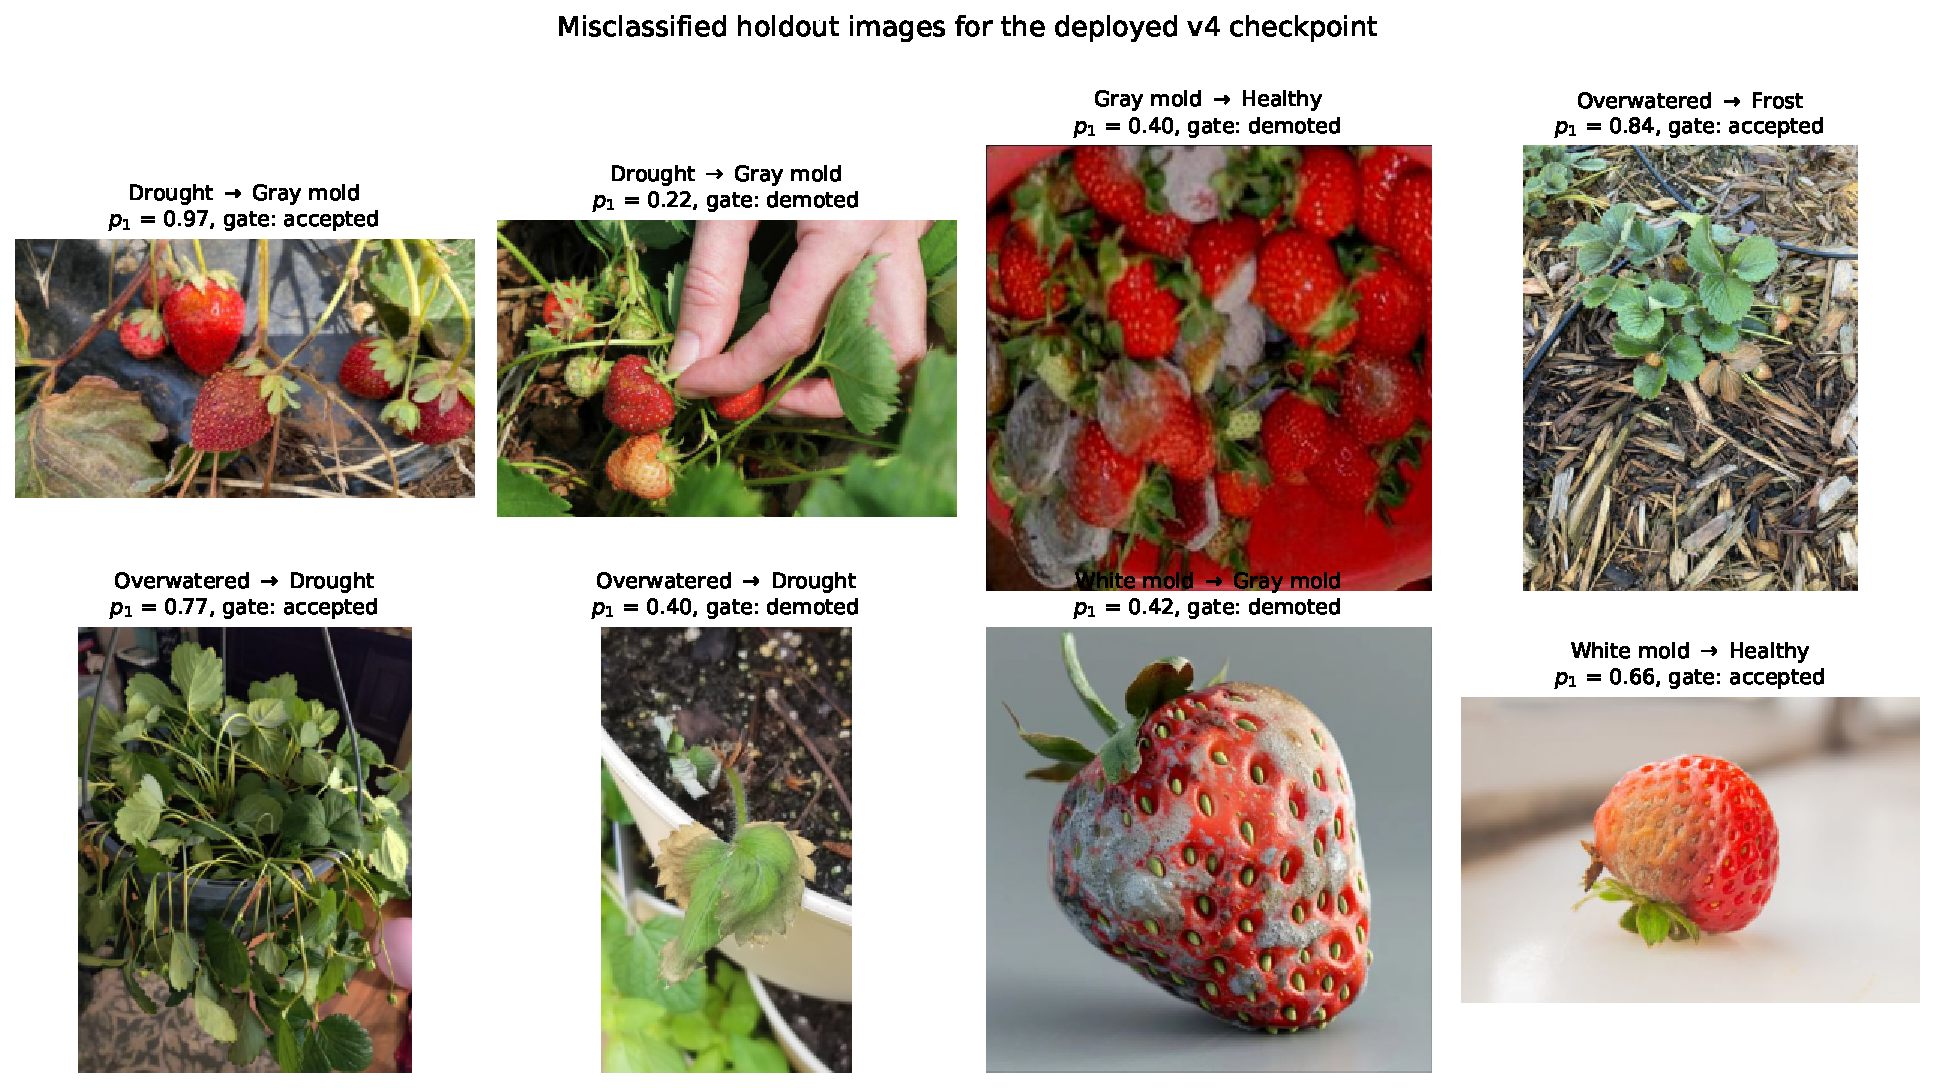
\includegraphics[width=\linewidth]{figures/generated/misclassification_grid.pdf}
\caption{The eight misclassified holdout images for the deployed v4
checkpoint, with ground-truth $\rightarrow$ predicted labels, the
calibrated top-1 probability $p_1$, and the deployed gate decision
(``demoted'' images are sent to \texttt{unknown} at runtime; ``accepted''
images are forwarded to the report writer).}
\label{fig:misclassification-grid}
\end{figure}

\subsection{Reproducibility Manifest}

The artifacts referenced in the main text are pinned as follows.

\paragraph{Source revision.}
Repository commit hash \texttt{6eaa403e021261f31f50e99a70c5b4a17944b497}.

\paragraph{Model weights (SHA-256).}
\begin{itemize}[leftmargin=1.3em]
\item ResNet-50 v4 classifier
(\texttt{plant\_diagnostic/models/resnet\_strawberry\_v4\_release10holdout.pth}):\\
\texttt{3d41c944c46b3f0bf5f356eb5e85df7f33afa69f2b121255421afc5558a569a2}.
\item RF-DETR Small detector
(\texttt{rfdetr\_parts/output/checkpoint\_best\_total.pth}):\\
\texttt{0274206eb1f851835193a1c30fc455d8cf2edaf98b5fb26dff16d785b45a431a}.
\end{itemize}

\paragraph{Evaluation artifacts.}
The classifier evaluation JSON is
\texttt{evaluation/holdout/resnet\_v4\_release10holdout\_full\_holdout.json}.
The dual-report pilot summary and per-record audit are
\texttt{evaluation/stage2\_pilot/dual\_report\_focus20\_tight/}
\texttt{dual\_report\_focus20\_tight\_summary.json} and
\texttt{...\_audit.jsonl}.

\paragraph{Random seed.}
Both training pipelines fix \texttt{seed=42}. The bootstrap confidence
intervals reported in \S\ref{sec:results-classifier} use a percentile
bootstrap with 10{,}000 resamples and seed 42.

\paragraph{Build pipeline.}
All figures and tables in the manuscript are generated by the following
scripts operating on the artifacts above:
\begin{itemize}[leftmargin=1.3em]
\item \texttt{paper/scripts/build\_paper\_assets.py} -- pipeline figure,
dataset counts, classifier confusion matrix, accuracy/calibration
figure, dual-report pilot summary;
\item \texttt{paper/scripts/compute\_extra\_metrics.py} -- bootstrap
confidence intervals, acceptance-gate replay, per-image
misclassification table;
\item \texttt{paper/scripts/compute\_threshold\_sweep.py} -- threshold
sensitivity sweep, risk-coverage curve, selective-accuracy table;
\item \texttt{paper/scripts/compute\_mcnemar.py} -- McNemar paired test
between v3 and v4 holdout predictions;
\item \texttt{paper/scripts/render\_misclass\_grid.py} -- per-image
misclassification grid;
\item \texttt{paper/scripts/run\_rfdetr\_on\_holdout.py} -- detector
inference on the disease holdout, per-class firing-rate table and
heatmap, latency summary (run inside the \texttt{rfdetr} conda env).
\end{itemize}
